		\begin{enumerate}
			\item \begin{enumerate}
				\item \phantom{x}
				
				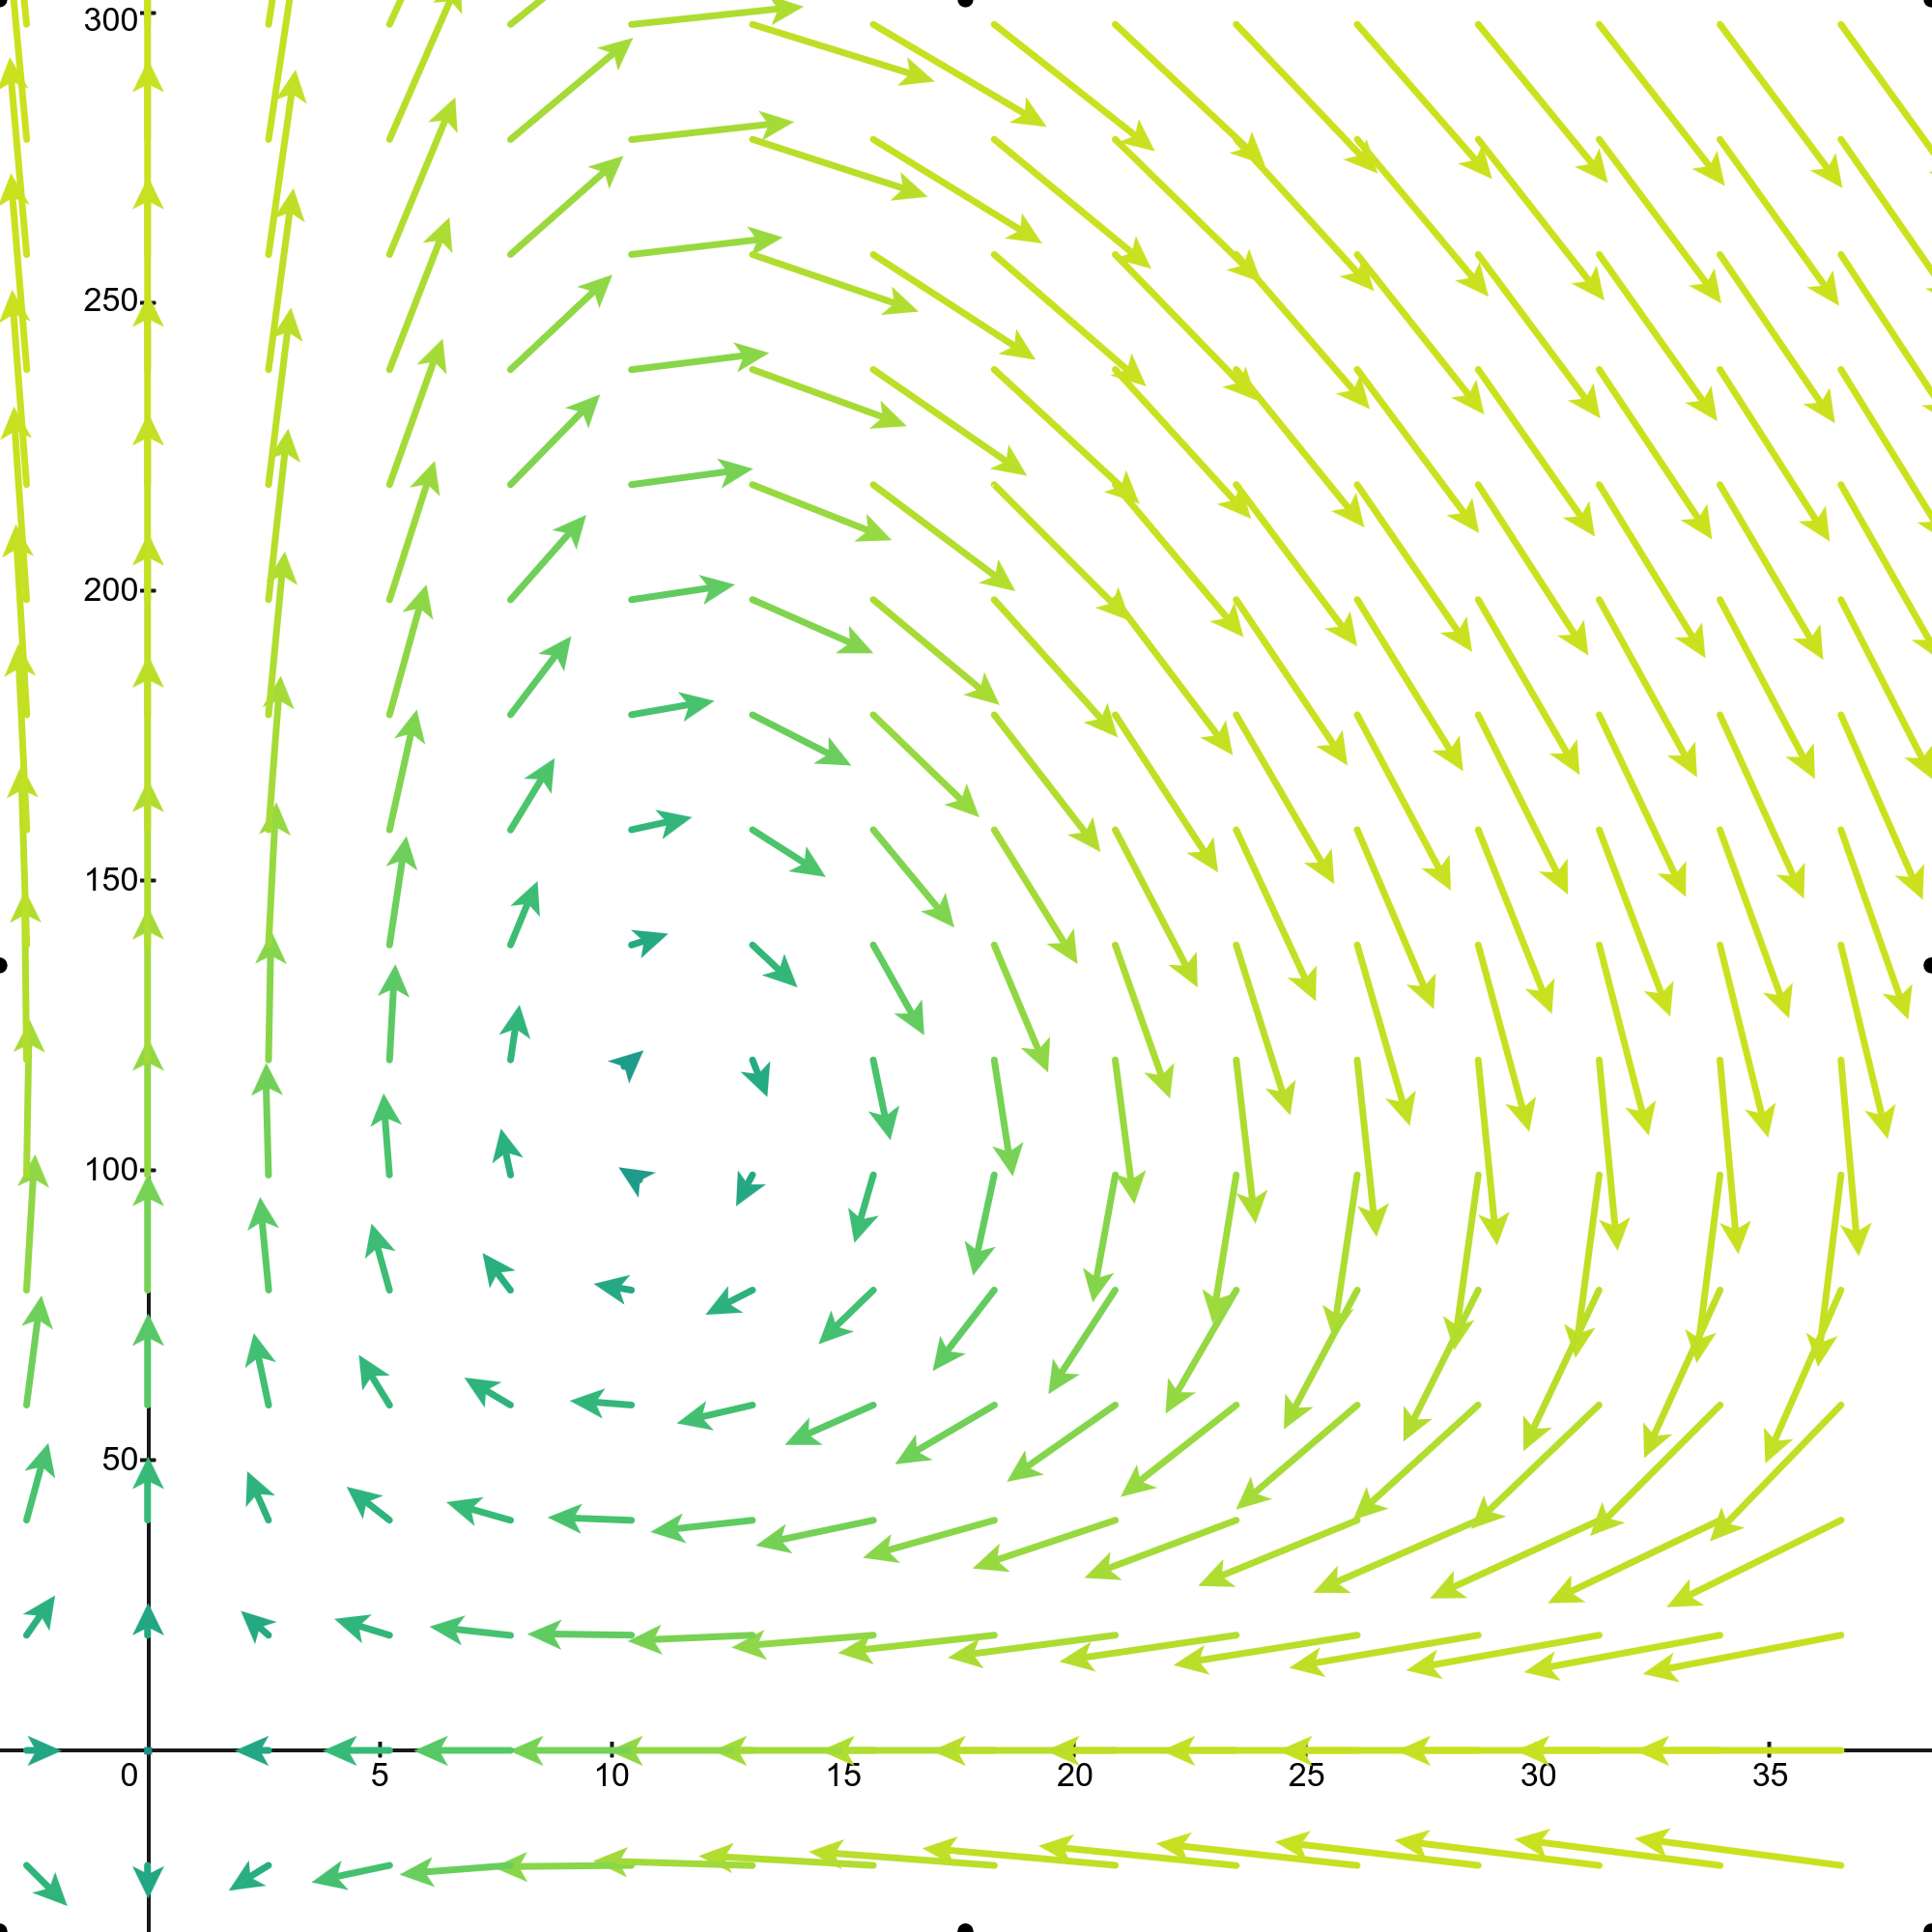
\includegraphics[width=3in]{resources/tutorial-02-1a.png}
					\item $\mathcal P=\Span\left\{\mat{1\\-1\\0},\mat{1\\0\\-1}, \mat{2\\-1\\-1}\right\}$.

				\item Arrows to the right of $F=11$ point down. That means as there are more foxes, the rabbit population decreases.
				Arrows to the left of $F=11$ point up, so as there are fewer foxes, there are more rabbits. If the arrows were oriented in the opposite direction,
				more foxes would lead to more rabbits, which is the opposite of what we would expect if the foxes ate the rabbits.
			\end{enumerate}
			\item ``The span of two \emph{linearly independent} vector $\vec p,\vec q\in \R^3$ is \emph{the} plane through
				the origin containing them.''
			\item \begin{enumerate}
				\item Positive $\Span\{\vec u,\vec v,\vec w\}=\{\vec x:\vec x=\alpha\vec u+\beta\vec v+\gamma \vec w\text{ for some }\alpha,\beta,\gamma\geq 0\}$.
				\item The \emph{positive span} of $\mat{1\\0}$ and $\mat{0\\1}$ is the first quadrant of the $xy$-plane, whereas
					the \emph{span} is the entire $xy$-plane.
				\item The positive span of linearly independent vectors could never be all of $\R^2$.
					Let $\vec u,\vec v\in \R^2$ be linearly independent.
					In this case, $\vec u\neq 0$ and $\vec u\neq t\vec v$ for any $t$.
					Therefore, the positive span of $\vec u$ and $\vec v$ cannot contain the vector $-\vec u\in \R^2$,
					and so the positive span of $\vec u$ and $\vec v$ is not all of $\R^2$.

					However, the positive span of a linearly dependent set could be all of $\R^2$. For example, $\left\{
						\mat{1\\0},\mat{0\\1},\mat{-1\\-1}\right\}$ has positive span equal to $\R^2$.
			\end{enumerate}
		\end{enumerate}
